\documentclass[student,noshadow]{ITRslides}
\usepackage{multimedia}

\usepackage[absolute,overlay]{textpos}
\renewcommand{\vec}[1]{\boldsymbol{#1}}
\addbibresource{ref.bib}
\graphicspath{{pics/}{logos/}}
\usepackage{psfrag}
\usepackage[percent]{overpic}
\usepackage{subcaption}
\usepackage{units}
\usepackage{tikz}
\usepackage{pgfplots}
\usepackage{booktabs}
\usetikzlibrary{positioning,shapes,fadings,decorations.pathmorphing,arrows}
\title{Object exploration using visual/haptic information by a human-robot team}
\presenter{Florian Wirnshofer, Benedikt Schmidt}

\supervisor{Denis Cehajic}
\typeofpres{Project Laboratory Cognitive Robotics and Control}

\definecolor{light-gray}{gray}{0.95}

\newcommand*\MyBlue{%
  \item[\color{blue}\scalebox{0.9}{\textbullet}]}
\newcommand*\MyRed{%
  \item[\color{red}\scalebox{0.9}{\textbullet}]}
%\nocite{*}

\renewcommand{\vec}[1]{\boldsymbol{#1}} 
% Alle indizes in Normalschrift ausser Läuferindizes
\newcommand{\scr}[1]{\mathrm{#1}} 

\makeatletter
\newif\iftikz@shading@path

\tikzset{
    % There are three circumstances in which the fading sep is needed:
    % 1. Arrows which do not update the bounding box (which is most of them).
    % 2. Line caps/joins and mitres that extend outside the natural bounding 
    %    box of the path (these are not calculated by PGF).
    % 3. Other reasons that haven't been anticipated.
    fading xsep/.store in=\pgfpathfadingxsep,
    fading ysep/.store in=\pgfpathfadingysep,
    fading sep/.style={fading xsep=#1, fading ysep=#1},
    fading sep=0.0cm,
    shading path/.code={%
        % Prevent this stuff happning recursively.
        \iftikz@shading@path%
        \else%
            \tikz@shading@pathtrue%
            % \tikz@addmode installs the `modes' (e.g., fill, draw, shade) 
            % to be applied to the path. It isn't usualy for doing more
            % changes to the path's construction.
            \tikz@addmode{%
                \pgfgetpath\pgf@currentfadingpath%
                % Get the boudning box of the current path size including the fading sep
                \pgfextract@process\pgf@fadingpath@southwest{\pgfpointadd{\pgfqpoint{\pgf@pathminx}{\pgf@pathminy}}%
                    {\pgfpoint{-\pgfpathfadingxsep}{-\pgfpathfadingysep}}}%%
                \pgfextract@process\pgf@fadingpath@northeast{\pgfpointadd{\pgfqpoint{\pgf@pathmaxx}{\pgf@pathmaxy}}%
                    {\pgfpoint{\pgfpathfadingxsep}{\pgfpathfadingysep}}}%
                % Clear the path
                \pgfsetpath\pgfutil@empty%                          
                % Interrupt the path and picture to create a fading.
                \pgfinterruptpath%
                \pgfinterruptpicture%
                    \begin{tikzfadingfrompicture}[name=.]
                        \path [shade=none,fill=none, #1] \pgfextra{%
                            % Set the softpath. Any transformations in #1 will have no effect.
                            % This will *not* update the bounding box...
                            \pgfsetpath\pgf@currentfadingpath%
                            % ...so it is done manually.
                            \pgf@fadingpath@southwest
                            \expandafter\pgf@protocolsizes{\the\pgf@x}{\the\pgf@y}%
                            \pgf@fadingpath@northeast%
                            \expandafter\pgf@protocolsizes{\the\pgf@x}{\the\pgf@y}%
                        };
                        % Now get the bounding of the picture.
                        \xdef\pgf@fadingboundingbox@southwest{\noexpand\pgfqpoint{\the\pgf@picminx}{\the\pgf@picminy}}%
                        \xdef\pgf@fadingboundingbox@northeast{\noexpand\pgfqpoint{\the\pgf@picmaxx}{\the\pgf@picmaxy}}%
                        %
                    \end{tikzfadingfrompicture}%
                \endpgfinterruptpicture%
                \endpgfinterruptpath%
                % Install a rectangle that covers the shaded/faded path picture.                                
                \pgfpathrectanglecorners{\pgf@fadingboundingbox@southwest}{\pgf@fadingboundingbox@northeast}%
                % Make the fading happen.
                \def\tikz@path@fading{.}%
                \tikz@mode@fade@pathtrue%
                \tikz@fade@adjustfalse%10pt
                % Shift the fading to the mid point of the rectangle
                \pgfpointscale{0.5}{\pgfpointadd{\pgf@fadingboundingbox@southwest}{\pgf@fadingboundingbox@northeast}}%
                \edef\tikz@fade@transform{shift={(\the\pgf@x,\the\pgf@y)}}%
            }%
        \fi%
    }
}

%%%%%%%%%%%%%%%%%%%%%%%%%%%%%%%%%%%%%%%%%%%%%%%%%%%%%%%%%%%%%%%%%%%%%%%%%%%%%%%%

\begin{document}


\begin{frame}
    \titlepage
\end{frame}

%%%%%%%%%%%%%%%%%%%%%%%%%%%%%%%%%%%%%%%%%%%%%%%%%%%%%%%%%%%%%%%%%%%%%%%%%%%%%%%%
%INTRODUCTION , MOTIVATION
%%%%%%%%%%%%%%%%%%%%%%%%%%%%%%%%%%%%%%%%%%%%%%%%%%%%%%%%%%%%%%%%%%%%%%%%%%%%%%%%
\begin{frame}
	\frametitle{Content}
	\tableofcontents
\end{frame}

\section{Online Load Estimation}
\begin{frame}
	%Benedikt
	\frametitle{Task}
	\begin{block}{Goal}
			Human-Robot cooperative estimation of load uncertainties.
	\end{block}
	\vspace{2mm}
	\begin{block}{Key-Questions}
			\begin{itemize}
				\item How to fuse and process sensor feedback, resulting in a reliable load-identification?
				\item How should the agents excite the load?
				\item How to exchange information between agents?
			\end{itemize}	   
	\end{block}	
\end{frame}

\begin{frame}
	%Florian
	\frametitle{Online Load Estimation}

	\begin{columns}
		\centering
		 	\begin{column}{0.25\textwidth}
			\begin{figure}
			\centering
				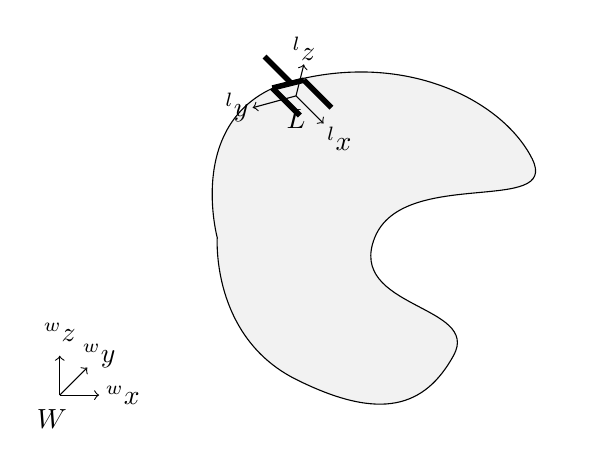
\begin{tikzpicture}
	% world frame
	\draw[arrows=->,line width=0.4pt] (0, 0) -- (0.5, 0);
	\draw[arrows=->,line width=0.4pt] (0, 0) -- (0.35, 0.35);
	\draw[arrows=->,line width=0.4pt] (0, 0) -- (0, 0.5);
	\node at (0.8, 0) {$^wx$};
	\node at (0.5, 0.5) {$^wy$};
	\node at (0, 0.8) {$^wz$};
	\node at (-0.1, -0.3) {$W$};
	
	% load
	\draw[fill,light-gray,draw=black] plot[smooth, tension=1.3] coordinates {(2, 2) (3, 4) (6, 3) (4, 2) (5, 0.5) (3, 0.2) (2, 2)};
	
	% load frame
	\draw[arrows=->,line width=0.4pt] (3, 3.8) -- (3.35, 3.45);
	\draw[arrows=->,line width=0.4pt] (3, 3.8) -- (2.45, 3.65);
	\draw[arrows=->,line width=0.4pt] (3, 3.8) -- (3.1, 4.2);
	\node at (3.55, 3.25) {$^lx$};
	\node at (2.25, 3.65) {$^ly$};
	\node at (3.1, 4.4) {$^lz$};
	\node at (3, 3.5) {$L$};
	
	% gripper
	\draw[draw=black,line width=2pt] (3.1, 4) -- (3.45, 3.65);
	\draw[draw=black,line width=2pt] (2.7, 3.9) -- (3.05, 3.55);
	\draw[draw=black,line width=2pt] (3.1, 4) -- (2.7, 3.9);
	\draw[draw=black,line width=2pt] (2.6, 4.3) -- (2.95, 3.95);
\end{tikzpicture} 
			\end{figure}
		 	\end{column}
		 		
		 	\begin{column}{0.75\textwidth}
			Model:\\ \cite{literaturstelle2}\\
			%\vspace{0.1cm}
			\[^\scr{L}\vec{F} = m {^\scr{W}}\vec{\ddot{p}} + m ^\scr{L}\vec{g} + ^\scr{L}\vec{\dot{\omega}} \times m ^\scr{L}\vec{c} + ^\scr{L}\vec{\omega} \times (^\scr{L}\vec{\omega} \times m ^\scr{L}\vec{c})\]
			\[^\scr{L}\vec{N} = ^\scr{L}\vec{I} ^\scr{L}\vec{\dot{\omega}} + ^\scr{L}\vec{\omega} \times (^\scr{L}\vec{I} ^\scr{L}\vec{\omega}) + m ^\scr{L}\vec{c} \times {^\scr{W}}\vec{\ddot{p}} + m ^\scr{L}\vec{c} \times ^\scr{L}\vec{g}\]
			
			\vspace{0.1cm}
			$\vec{\ddot{p}}$ EEF acceleration\\
			$m$ Object mass\\
			$\vec{I}$  Object inertia tensor
		 	\end{column}
	\end{columns}
	 		\vspace{0.2cm}
			RLS Estimation-Parameters: \\
			$\vec{\Theta} = [m, m c_\scr{x}, m c_\scr{y}, m c_\scr{z}, I_\scr{xx}, I_\scr{xy}, I_\scr{xz}, I_\scr{yy},I_\scr{yz}, I_\scr{zz}]^\scr{T}$ \\
\end{frame}

\begin{frame}
	%Florian
	\frametitle{Cooperative Online Load Estimation}
	\begin{columns}
			\begin{column}{0.5\textwidth}
				\begin{figure}
					\centering
					\resizebox{4cm}{!}{
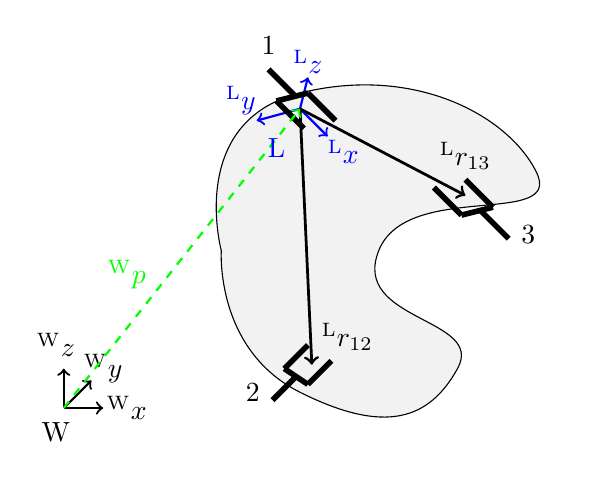
\begin{tikzpicture}
	% world frame
	\draw[arrows=->,line width=0.8pt] (0, 0) -- (0.5, 0);
	\draw[arrows=->,line width=0.8pt] (0, 0) -- (0.35, 0.35);
	\draw[arrows=->,line width=0.8pt] (0, 0) -- (0, 0.5);
	\node at (0.8, 0) {{$^\mathrm{W}x$}};
	\node at (0.5, 0.5) {{$^\mathrm{W}y$}};
	\node at (-0.1, 0.8) {{$^\mathrm{W}z$}};
	\node at (-0.1, -0.3) {W};	
	% load
	\draw[fill,light-gray,draw=black] plot[smooth, tension=1.3] coordinates {(2, 2) (3, 4) (6, 3) (4, 2) (5, 0.5) (3, 0.2) (2, 2)};
	
	% load frame
	\draw[draw=blue,arrows=->,line width=0.8pt] (3, 3.8) -- (3.35, 3.45);
	\draw[draw=blue,arrows=->,line width=0.8pt] (3, 3.8) -- (2.45, 3.65);
	\draw[draw=blue,arrows=->,line width=0.8pt] (3, 3.8) -- (3.1, 4.2);
	\node[text=blue] at (3.55, 3.25) {{$^\mathrm{L}x$}};
	\node[text=blue] at (2.25, 3.9) {{$^\mathrm{L}y$}};
	\node[text=blue] at (3.1, 4.4) {{$^\mathrm{L}z$}};
	
		
	
	
	% gripper one
	\draw[draw=black,line width=2pt] (3.1, 4) -- (3.45, 3.65);
	\draw[draw=black,line width=2pt] (2.7, 3.9) -- (3.05, 3.55);
	\draw[draw=black,line width=2pt] (3.1, 4) -- (2.7, 3.9);
	\draw[draw=black,line width=2pt] (2.6, 4.3) -- (2.95, 3.95);
	\node at (2.6, 4.6) {$1$};
	
	% gripper two
	\draw[draw=black,line width=2pt] (2.8, 0.5) -- (3.1, 0.3);
	\draw[draw=black,line width=2pt] (2.8, 0.5) -- (3.1, 0.8);
	\draw[draw=black,line width=2pt] (3.1, 0.3) -- (3.4, 0.6);
	\draw[draw=black,line width=2pt] (2.65, 0.1) -- (2.95, 0.4);
	\node at (2.4, 0.2) {$2$};
	
	% gripper three
	\draw[draw=black,line width=2pt] (5.1, 2.9) -- (5.45, 2.55);
	\draw[draw=black,line width=2pt] (4.7, 2.8) -- (5.05, 2.45);
	\draw[draw=black,line width=2pt] (5.45, 2.55) -- (5.05, 2.45);
	\draw[draw=black,line width=2pt] (5.65, 2.15) -- (5.3, 2.5);
	\node at (5.9, 2.2) {$3$};
	
	% grasping offsets
	\draw[arrows=->,line width=1pt] (3, 3.8) -- (3.15, 0.55);
	\node at (3.6, 0.9) {$^\scr{L}\vec{r}_{12}$};
	\draw[arrows=->,line width=1pt] (3, 3.8) -- (5.1, 2.7);
	\node at (5.1, 3.2) {$^\scr{L}\vec{r}_{13}$};
	
	\draw[->,thick,dashed,green](0, 0) -- (3, 3.8);
	\node[text=blue] at (2.7, 3.3) {L};
	\node[text=green] at (0.8, 1.7) {$^\scr{W}\vec{p}$};
\end{tikzpicture}
}
				\end{figure}	
		 	\end{column}
		 	\begin{column}{0.5\textwidth}
		 	$^\scr{L}\vec{F}_i$: Forces acting at grasping point $i$, measured w.r.t. the EEF frame L.\\ \vspace{0.3cm}
		 	$^\scr{L}\vec{N}_i$: Torques acting at grasping point $i$, measured w.r.t. the EEF frame L.\\
		 	\end{column}
	\end{columns}

\begin{align*} 
\sum_{i = 1}^{n}  {^\scr{L}}\vec{F}_{i} &=  f\left(^\scr{W}\vec{\ddot{p}},^\scr{L}\vec{\omega},^\scr{L}\vec{\dot{\omega}},^\scr{L}\vec{c},m\right) \\ 
\sum_{i = 1}^n {^\scr{L}}\vec{N}_{i} + \sum_{i = 2}^n {^\scr{L}}\vec{r}_{1i} \times {^\scr{L}}\vec{F}_{i} &= f\left({^\scr{W}}\vec{\ddot{p}},{^\scr{L}}\vec{\omega}{^\scr{L}},\vec{\dot{\omega}},{^\scr{L}}\vec{c},{^\scr{L}}\vec{I},m\right)
\end{align*}
\end{frame}

\begin{frame}
	%Florian
	\frametitle{Persistent Excitation}
	\simpleblock{
	\begin{small}
		\begin{center}
			RLS convergence prerequisites
		\end{center}
	\end{small}
	}
	\vspace{1cm}	
	\begin{itemize}
		\item Reference trajectory must be persistently exciting(PE)
		\item Non-zero acceleration of EEF in 6-DoF \cite{literaturstelle3}
	\end{itemize}
	\vspace{1cm}
	\textsc{Challenge}: Satisfaction of actuator limits, especially when trying to identify big objects.
\end{frame}

\section{Signal Processing}
\begin{frame}
	%Florian
	\frametitle{Acquisition}
	\begin{columns}
	\begin{column}{0.35\textwidth}
				\begin{figure}
					\centering
					\resizebox{4cm}{!}{
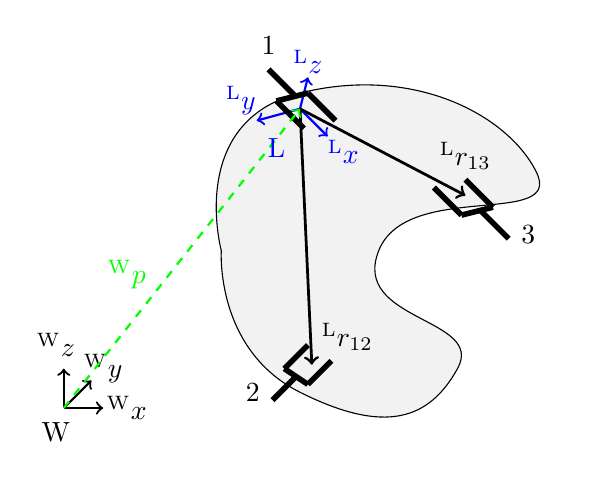
\begin{tikzpicture}
	% world frame
	\draw[arrows=->,line width=0.8pt] (0, 0) -- (0.5, 0);
	\draw[arrows=->,line width=0.8pt] (0, 0) -- (0.35, 0.35);
	\draw[arrows=->,line width=0.8pt] (0, 0) -- (0, 0.5);
	\node at (0.8, 0) {{$^\mathrm{W}x$}};
	\node at (0.5, 0.5) {{$^\mathrm{W}y$}};
	\node at (-0.1, 0.8) {{$^\mathrm{W}z$}};
	\node at (-0.1, -0.3) {W};	
	% load
	\draw[fill,light-gray,draw=black] plot[smooth, tension=1.3] coordinates {(2, 2) (3, 4) (6, 3) (4, 2) (5, 0.5) (3, 0.2) (2, 2)};
	
	% load frame
	\draw[draw=blue,arrows=->,line width=0.8pt] (3, 3.8) -- (3.35, 3.45);
	\draw[draw=blue,arrows=->,line width=0.8pt] (3, 3.8) -- (2.45, 3.65);
	\draw[draw=blue,arrows=->,line width=0.8pt] (3, 3.8) -- (3.1, 4.2);
	\node[text=blue] at (3.55, 3.25) {{$^\mathrm{L}x$}};
	\node[text=blue] at (2.25, 3.9) {{$^\mathrm{L}y$}};
	\node[text=blue] at (3.1, 4.4) {{$^\mathrm{L}z$}};
	
		
	
	
	% gripper one
	\draw[draw=black,line width=2pt] (3.1, 4) -- (3.45, 3.65);
	\draw[draw=black,line width=2pt] (2.7, 3.9) -- (3.05, 3.55);
	\draw[draw=black,line width=2pt] (3.1, 4) -- (2.7, 3.9);
	\draw[draw=black,line width=2pt] (2.6, 4.3) -- (2.95, 3.95);
	\node at (2.6, 4.6) {$1$};
	
	% gripper two
	\draw[draw=black,line width=2pt] (2.8, 0.5) -- (3.1, 0.3);
	\draw[draw=black,line width=2pt] (2.8, 0.5) -- (3.1, 0.8);
	\draw[draw=black,line width=2pt] (3.1, 0.3) -- (3.4, 0.6);
	\draw[draw=black,line width=2pt] (2.65, 0.1) -- (2.95, 0.4);
	\node at (2.4, 0.2) {$2$};
	
	% gripper three
	\draw[draw=black,line width=2pt] (5.1, 2.9) -- (5.45, 2.55);
	\draw[draw=black,line width=2pt] (4.7, 2.8) -- (5.05, 2.45);
	\draw[draw=black,line width=2pt] (5.45, 2.55) -- (5.05, 2.45);
	\draw[draw=black,line width=2pt] (5.65, 2.15) -- (5.3, 2.5);
	\node at (5.9, 2.2) {$3$};
	
	% grasping offsets
	\draw[arrows=->,line width=1pt] (3, 3.8) -- (3.15, 0.55);
	\node at (3.6, 0.9) {$^\scr{L}\vec{r}_{12}$};
	\draw[arrows=->,line width=1pt] (3, 3.8) -- (5.1, 2.7);
	\node at (5.1, 3.2) {$^\scr{L}\vec{r}_{13}$};
	
	\draw[->,thick,dashed,green](0, 0) -- (3, 3.8);
	\node[text=blue] at (2.7, 3.3) {L};
	\node[text=green] at (0.8, 1.7) {$^\scr{W}\vec{p}$};
\end{tikzpicture}
}
				\end{figure}	
		 	\end{column}
		 	\begin{column}{0.65\textwidth}
		 	\begin{tabular}{llr}
				\toprule
				Information    & Tool & Frame Rate $\left[\mathrm{Hz}\right]$ \\
				\midrule
				${^\scr{L}}\vec{F}_{i},{^\scr{L}}\vec{N}_{i}$      & \textsc{JR3}    & 8000 $\rightarrow$ 100      \\
				          & \textsc{Qualisys}        & 100       \\
				$^\scr{L}\vec{\omega}$       & \textsc{Qualisys}     & 100      \\
				$^\scr{W}\vec{p}$       & \textsc{Qualisys}     & 100      \\
				$^\scr{L}\vec{r}_{1i}$ & \textsc{Qualisys}      & 100       \\
				\bottomrule
			\end{tabular}
		 	%${^\scr{L}}\vec{F}_{i}$: Force measured at $i$-th grasping point w.r.t. the EEF frame L.\\ \vspace{0.3cm}
		 	%${^\scr{L}}\vec{N}_{i}$: Torque measured at $i$-th grasping point w.r.t. the EEF frame L.
		 	\end{column}
	\end{columns}
\end{frame}

\begin{frame}
	%Florian
	\frametitle{Processing}
	
	\textsc{Main Issue}: Noise prone first and second derivatives\\
	\textsc{Solution}: Butterworth lowpass filter (Order:3, $\omega_\mathrm{CutOff} = 30 \mathrm{Hz}$)
	\begin{figure}
		\centering
		% This file was created by matlab2tikz.
%
%The latest updates can be retrieved from
%  http://www.mathworks.com/matlabcentral/fileexchange/22022-matlab2tikz
%where you can also make suggestions and rate matlab2tikz.
%
\begin{tikzpicture}

\begin{axis}[%
width=4.822222in,
height=3.803333in,
at={(0.808889in,0.513333in)},
scale only axis,
every outer x axis line/.append style={black},
every x tick label/.append style={font=\color{black}},
xmin=0,
xmax=1,
xtick={\empty},
xlabel={Frequency  (Hz)},
every outer y axis line/.append style={black},
every y tick label/.append style={font=\color{black}},
ymin=0,
ymax=1,
ytick={\empty},
hide axis,
title={Bode Diagram},
axis x line*=bottom,
axis y line*=left
]
\end{axis}

\begin{axis}[%
width=4.688889in,
height=1.620456in,
at={(0.942222in,0.513333in)},
scale only axis,
separate axis lines,
every outer x axis line/.append style={white!40!black},
every x tick label/.append style={font=\color{white!40!black}},
xmode=log,
xmin=0.1,
xmax=100,
xminorticks=true,
every outer y axis line/.append style={white!40!black},
every y tick label/.append style={font=\color{white!40!black}},
ymin=-3.6,
ymax=363.6,
ytick={  0,  90, 180, 270, 360},
ylabel={Phase (deg)}
]
\addplot [color=blue,solid,forget plot]
  table[row sep=crcr]{%
1.59154943091895e-21	360\\
6.35930251634695e-16	360\\
6.35930251634695e-11	359.999999999834\\
6.35930251634695e-07	359.999998336691\\
0.000635930251634694	359.998336690658\\
0.0635930251634694	359.833668786141\\
0.635930251634694	358.336410883883\\
0.706264699851281	358.152343900741\\
0.784378200240987	357.947892097914\\
0.871131122853577	357.7207909569\\
0.967478995427185	357.46852181884\\
1.07448302791281	357.188282409868\\
1.1933218010205	356.87695359805\\
1.32530424752914	356.531061774888\\
1.47188406934049	356.146736115439\\
1.63467574907224	355.719659789129\\
1.81547233254737	355.245013952751\\
2.01626517804255	354.717413035915\\
2.23926588982093	354.130829396386\\
2.48693067753298	353.478504834158\\
2.76198740978868	352.752845645595\\
3.06746565987866	351.945296780563\\
3.4067300745787	351.046189101585\\
3.78351743357351	350.044551534123\\
4.20197780768557	348.927876738574\\
4.66672026924043	347.681824362639\\
5.18286365803888	346.289839220756\\
5.75609296209056	344.732651735236\\
6.39272193410647	342.987612769522\\
7.09976263343105	341.027791426629\\
7.88500265937334	338.820727059093\\
8.75709092661294	336.32666610541\\
9.72563292744169	333.496013160743\\
10.8012965300935	330.265551690599\\
11.9959294784633	326.552681136146\\
13.322689887398	322.246351856128\\
14.7961911708833	317.19231266668\\
15.9695747210457	312.922382668778\\
17.548238595208	306.760365406415\\
19.1225693616108	300.031633416154\\
20.6801127162529	292.660608953727\\
22.2098911830924	284.566156664673\\
23.702481035695	275.676366907489\\
25.1500210470845	265.95558963511\\
26.5461672933504	255.443876013087\\
27.8860076595316	244.297947756234\\
29.1659483942505	232.807385617978\\
30.3835833549209	221.357724560447\\
31.537554726176	210.342599955522\\
32.7353540393206	199.069108827239\\
34.1020063761277	186.759354198447\\
35.6672554296806	173.685797201372\\
36.4246000866322	167.787386902943\\
36.4246861899723	167.786731973396\\
38.0740555500801	155.858391363481\\
38.074145552533	155.857772391694\\
39.5775946537461	145.945535088941\\
39.5776882103832	145.944943021877\\
40.9410101677892	137.598527807931\\
40.9411069473753	137.597953795271\\
42.17174536179	130.480486486464\\
42.171845050685	130.479923547263\\
43.2782974810962	124.348396895314\\
43.2783997857463	124.347839956494\\
44.2697385186491	119.025786979014\\
44.2698431669457	119.025232497305\\
45.1553421200665	114.381259170123\\
45.1554488618227	114.380704734087\\
45.9443025817414	110.313853755963\\
45.9444111885045	110.313297766053\\
46.64553114355	106.743525554444\\
46.6456414079324	106.742966986807\\
47.2675153508705	103.605013485771\\
47.2676270855482	103.604451723064\\
47.8182285855702	100.843867232068\\
47.8183416220672	100.843301943209\\
48.3050785401915	98.4138276603642\\
48.3051927275428	98.4132587148164\\
48.7348851706872	96.2750577295048\\
48.7350003740493	96.2744851357593\\
49.1138803507211	94.3929122776111\\
49.1139964499818	94.3923361386858\\
49.4477229773757	92.7370537732843\\
49.4478398657999	92.7364742543389\\
49.7415246053379	91.2807939013141\\
49.7416421882737	91.28021120601\\
49.9998818063392	19.4716413673132\\
50	1.27222187258541e-13\\
};
\addplot [color=black,solid,forget plot]
  table[row sep=crcr]{%
50	-1e+99\\
50	-1e+96\\
50	-1e+93\\
50	-1e+90\\
50	-1e+87\\
50	-1e+84\\
50	-1e+81\\
50	-1e+78\\
50	-1e+75\\
50	-1e+72\\
50	-1e+69\\
50	-1e+66\\
50	-1e+63\\
50	-1e+60\\
50	-1e+57\\
50	-1e+54\\
50	-1e+51\\
50	-1e+48\\
50	-1e+45\\
50	-1e+42\\
50	-1e+39\\
50	-1e+36\\
50	-1e+33\\
50	-1e+30\\
50	-1e+27\\
50	-1e+24\\
50	-1e+21\\
50	-1e+18\\
50	-1e+15\\
50	-1000000000000\\
50	-1000000000\\
50	-1000000\\
50	-1000\\
50	-1\\
50	0\\
50	1\\
50	1000\\
50	1000000\\
50	1000000000\\
50	1000000000000\\
50	1e+15\\
50	1e+18\\
50	1e+21\\
50	1e+24\\
50	1e+27\\
50	1e+30\\
50	1e+33\\
50	1e+36\\
50	1e+39\\
50	1e+42\\
50	1e+45\\
50	1e+48\\
50	1e+51\\
50	1e+54\\
50	1e+57\\
50	1e+60\\
50	1e+63\\
50	1e+66\\
50	1e+69\\
50	1e+72\\
50	1e+75\\
50	1e+78\\
50	1e+81\\
50	1e+84\\
50	1e+87\\
50	1e+90\\
50	1e+93\\
50	1e+96\\
50	1e+99\\
};
\end{axis}

\begin{axis}[%
width=4.688889in,
height=1.827322in,
at={(0.942222in,2.267122in)},
scale only axis,
separate axis lines,
every outer x axis line/.append style={white!40!black},
every x tick label/.append style={font=\color{white!40!black}},
xmode=log,
xmin=0.1,
xmax=100,
xtick={0.1,1,10,100},
xticklabels={\empty},
xminorticks=true,
every outer y axis line/.append style={white!40!black},
every y tick label/.append style={font=\color{white!40!black}},
ymin=-400,
ymax=0,
ylabel={Magnitude (dB)}
]
\addplot [color=blue,solid,forget plot]
  table[row sep=crcr]{%
1.59154943091895e-21	7.71461973242629e-15\\
6.35930251634695e-16	7.71461973242629e-15\\
6.35930251634695e-11	9.64327466553287e-15\\
6.35930251634695e-07	5.78596479931972e-15\\
0.000635930251634694	3.85730986621315e-15\\
0.0635930251634694	7.71461973242629e-15\\
0.635930251634694	-4.06396524230503e-11\\
0.706264699851281	-7.62840885694993e-11\\
0.784378200240987	-1.43189128199812e-10\\
0.871131122853577	-2.68775422826958e-10\\
0.967478995427185	-5.04543845135066e-10\\
1.07448302791281	-9.47181724249614e-10\\
1.1933218010205	-1.77834038943963e-09\\
1.32530424752914	-3.33924807930847e-09\\
1.47188406934049	-6.27117484532709e-09\\
1.63467574907224	-1.1779621634736e-08\\
1.81547233254737	-2.21317165458199e-08\\
2.01626517804255	-4.15933540647417e-08\\
2.23926588982093	-7.81964949364494e-08\\
2.48693067753298	-1.47075873477305e-07\\
2.76198740978868	-2.76777728992148e-07\\
3.06746565987866	-5.21208900336497e-07\\
3.4067300745787	-9.82317755912097e-07\\
3.78351743357351	-1.85326051475869e-06\\
4.20197780768557	-3.50082463327125e-06\\
4.66672026924043	-6.62344587179999e-06\\
5.18286365803888	-1.25556515550046e-05\\
5.75609296209056	-2.38581895228601e-05\\
6.39272193410647	-4.547048376482e-05\\
7.09976263343105	-8.69818997612663e-05\\
7.88500265937334	-0.000167158276943463\\
8.75709092661294	-0.00032308716012471\\
9.72563292744169	-0.000628964807169664\\
10.8012965300935	-0.001235480437394\\
11.9959294784633	-0.00245443475123012\\
13.322689887398	-0.00494602661761731\\
14.7961911708833	-0.0101484147713166\\
15.9695747210457	-0.017361700256594\\
17.548238595208	-0.0343876970631704\\
19.1225693616108	-0.0656346151624357\\
20.6801127162529	-0.121104183602466\\
22.2098911830924	-0.216428858139419\\
23.702481035695	-0.374803299112322\\
25.1500210470845	-0.628235900003408\\
26.5461672933504	-1.01644348711892\\
27.8860076595316	-1.58129384182944\\
29.1659483942505	-2.35624389693408\\
30.3835833549209	-3.35444252223818\\
31.537554726176	-4.56269256094041\\
32.7353540393206	-6.09537340663536\\
34.1020063761277	-8.18004807600633\\
35.6672554296806	-10.9787584550037\\
36.4246000866322	-12.4833195625616\\
36.4246861899723	-12.483496154474\\
38.0740555500801	-16.1040848325914\\
38.074145552533	-16.1042958637569\\
39.5775946537461	-19.8584578655177\\
39.5776882103832	-19.8587067687513\\
40.9410101677892	-23.7232286714163\\
40.9411069473753	-23.7235214262871\\
42.17174536179	-27.7012663006636\\
42.171845050685	-27.7016113148233\\
43.2782974810962	-31.809373239691\\
43.2783997857463	-31.8097816124337\\
44.2697385186491	-36.0736382322672\\
44.2698431669457	-36.0741244308575\\
45.1553421200665	-40.5289674139026\\
45.1554488618227	-40.5295504570207\\
45.9443025817414	-45.221322777476\\
45.9444111885045	-45.2220281686503\\
46.64553114355	-50.2125716534366\\
46.6456414079324	-50.2134345726873\\
47.2675153508705	-55.5891006370933\\
47.2676270855482	-55.5901714388661\\
47.8182285855702	-61.47726673906\\
47.8183416220672	-61.4786210455367\\
48.3050785401915	-68.0730526499445\\
48.3051927275428	-68.074811544088\\
48.7348851706872	-75.705147725228\\
48.7350003740493	-75.7075231864255\\
49.1138803507211	-84.9903955635315\\
49.1139964499818	-84.9938116233761\\
49.4477229773757	-97.3146366692462\\
49.4478398657999	-97.3201534178872\\
49.7415246053379	-117.100944911782\\
49.7416421882737	-117.112802013281\\
49.9998818063392	-307.948570481751\\
50	-308.460086867919\\
};
\addplot [color=black,solid,forget plot]
  table[row sep=crcr]{%
50	-1980\\
50	-1920\\
50	-1860\\
50	-1800\\
50	-1740\\
50	-1680\\
50	-1620\\
50	-1560\\
50	-1500\\
50	-1440\\
50	-1380\\
50	-1320\\
50	-1260\\
50	-1200\\
50	-1140\\
50	-1080\\
50	-1020\\
50	-960\\
50	-900\\
50	-840\\
50	-780\\
50	-720\\
50	-660\\
50	-600\\
50	-540\\
50	-480\\
50	-420\\
50	-360\\
50	-300\\
50	-240\\
50	-180\\
50	-120\\
50	-60\\
50	0\\
50	60\\
50	120\\
50	180\\
50	240\\
50	300\\
50	360\\
50	420\\
50	480\\
50	540\\
50	600\\
50	660\\
50	720\\
50	780\\
50	840\\
50	900\\
50	960\\
50	1020\\
50	1080\\
50	1140\\
50	1200\\
50	1260\\
50	1320\\
50	1380\\
50	1440\\
50	1500\\
50	1560\\
50	1620\\
50	1680\\
50	1740\\
50	1800\\
50	1860\\
50	1920\\
50	1980\\
};
\end{axis}
\end{tikzpicture}%
	\end{figure}	
\end{frame}

\section{Experimental Results}
\begin{frame}
	%Benedikt
	\frametitle{Simulation Results with Noise ($P = \unit[0.05]{W}$)}
	\begin{center}
		Error of mass $m \left[\mathrm{kg}\right]$
		\begin{figure}
			\psfrag{x}[tr][br]{$t\left[\mathrm{s}\right]$}
			\psfrag{y1}[br][tr]{$\epsilon_\scr{Mass}$}
			\psfrag{y2}[br][tr]{$\epsilon_\scr{CoM}$}
			\psfrag{one}[c][Bc]{$0$}
			\psfrag{two}[c][Bc]{$1$}
			\psfrag{thr}[c][Bc]{$2$}
			\psfrag{fou}[c][Bc]{$3$}
			\psfrag{fiv}[c][Bc]{$4$}
			\psfrag{six}[c][Bc]{$5$}
			\psfrag{lllllllll}[Br][Bl]{$10^{-6}\  $}
			\psfrag{lllllllli}[Br][Bl]{$10^{-4}\  $}
			\psfrag{lllllllil}[Br][Bl]{$10^{-2}\  $}
			\psfrag{lllllllii}[Br][Bl]{$10^0\  $}
			\psfrag{llllllill}[Br][Bl]{$10^{-10}\  $}
			\psfrag{llllllili}[Br][Bl]{$10^{-5}\  $}
			\psfrag{lllllliil}[Br][Bl]{$10^0\  $}
			\psfrag{cerror1}[][]{\tiny $c_{x}$}
			\psfrag{cerror2}[][]{\tiny $c_{y}$}
			\psfrag{cerror3}[][]{\tiny $c_{z}$}
			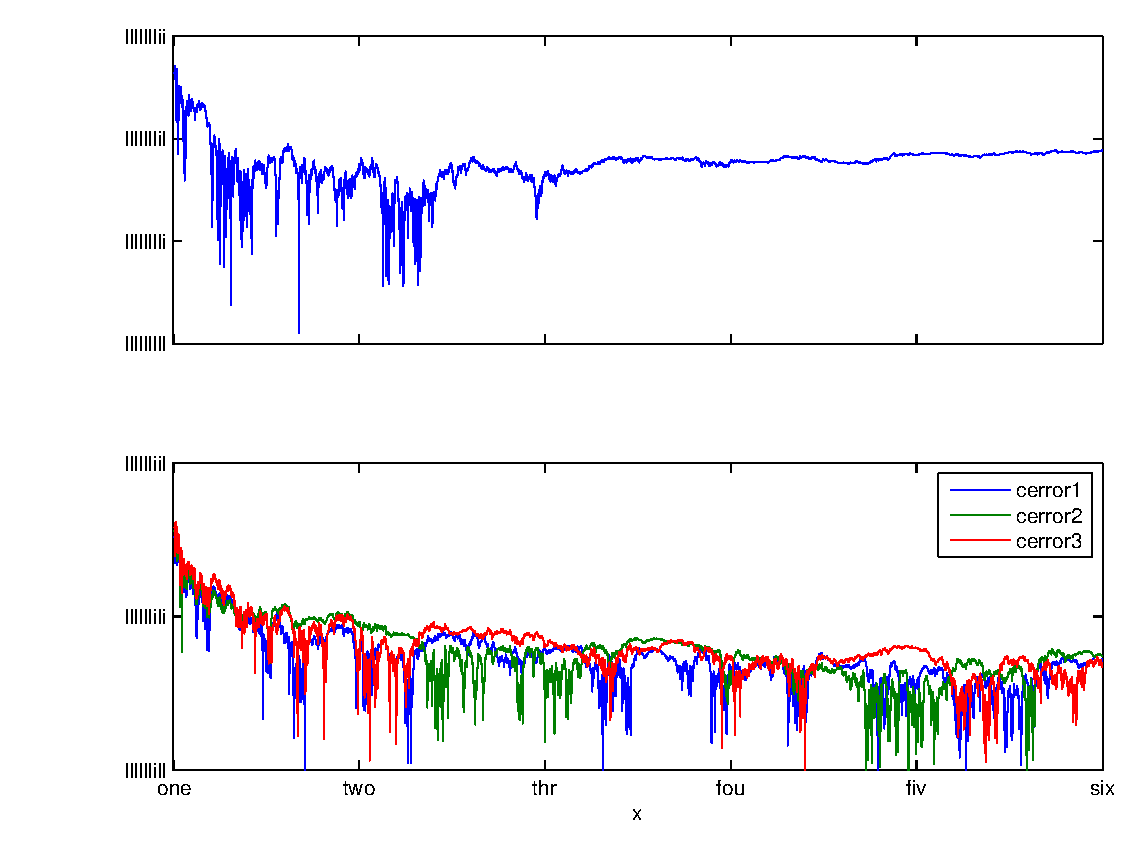
\includegraphics[width=0.6\textwidth]{fig/mass_multi_noise.eps}
		\end{figure}
		Error of center of gravity $\vec{c} \left[\mathrm{m}\right]$
	\end{center}
\end{frame}

\begin{frame}
	%Benedikt
	\frametitle{Simulation Results with Noise ($P = \unit[0.05]{W}$)}
	\begin{center}
		\centering
		\begin{figure}
			\psfrag{xaxis}[tr][br]{$t\left[\mathrm{s}\right]$}
			\psfrag{yaxis}[br][tr]{$\epsilon_{\scr{Inertia}}$}
			\psfrag{one}[c][Bc]{$0$}
			\psfrag{two}[c][Bc]{$1$}
			\psfrag{thr}[c][Bc]{$2$}
			\psfrag{fou}[c][Bc]{$3$}
			\psfrag{fiv}[c][Bc]{$4$}
			\psfrag{six}[c][Bc]{$5$}
			\psfrag{lllllllll}[Br][Bl]{$10^{-10}\  $}
			\psfrag{lllllllli}[Br][Bl]{$10^{-6}\  $}
			\psfrag{lllllllil}[Br][Bl]{$10^{-2}\  $}
			\psfrag{lllllllii}[Br][Bl]{$10^2\  $}
			\psfrag{Ierror1}[][]{\tiny \  $I_{xx}$}
			\psfrag{Ierror2}[][]{\tiny \  $I_{yy}$}
			\psfrag{Ierror3}[][]{\tiny \  $I_{zz}$}
			\psfrag{Ierror4}[][]{\tiny \  $I_{xy}$}
			\psfrag{Ierror5}[][]{\tiny \  $I_{xz}$}
			\psfrag{Ierror6}[][]{\tiny \  $I_{yz}$}
			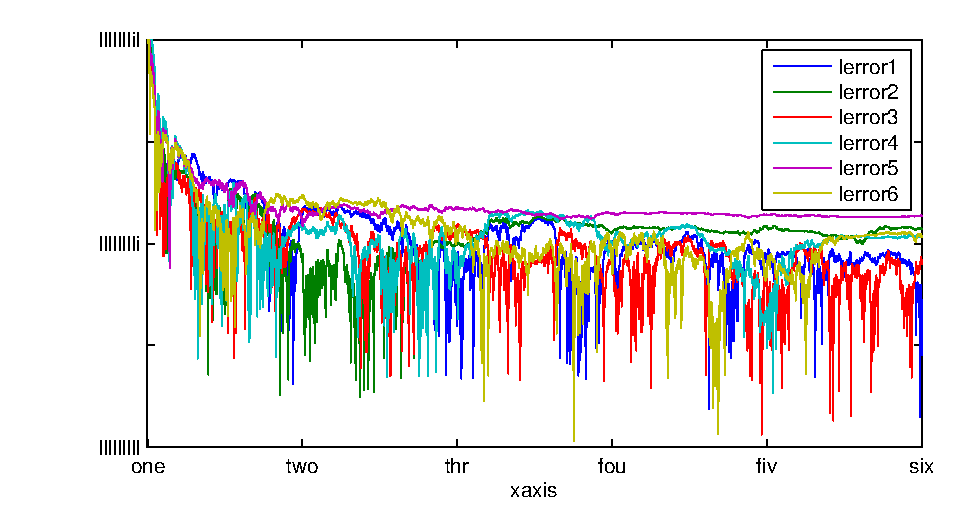
\includegraphics[width=0.6\textwidth]{fig/inertia_multi_noise.eps}
		\end{figure}
		\vspace{0.5cm}
		Error of inertias $I \left[\mathrm{kg} \cdot \mathrm{m}^2\right]$
	\end{center}
\end{frame}

\begin{frame}
	%Benedikt
	\frametitle{Estimation Results}
	\begin{center}
		Error of mass $m \left[\mathrm{kg}\right]$
		\begin{figure}
			\centering	
			\psfrag{xaxis}[tr][br]{$t\left[\mathrm{s}\right]$}
			\psfrag{yaxism}[bc][tr]{}
			\psfrag{yaxisc}[bc][tr]{}
			\psfrag{one}[c][Bc]{$0$}
			\psfrag{two}[c][Bc]{$1$}
			\psfrag{thr}[c][Bc]{$2$}
			\psfrag{fou}[c][Bc]{$3$}
			\psfrag{fiv}[c][Bc]{$4$}
			\psfrag{six}[c][Bc]{$5$}
			\psfrag{sev}[c][Bc]{$6$}
			\psfrag{eig}[c][Bc]{$7$}
			\psfrag{lllllllll}[Br][Bl]{$-0.3\  $}
			\psfrag{lllllllli}[Br][Bl]{$-0.15\ $}
			\psfrag{lllllllil}[Br][Bl]{$0\  $}
			\psfrag{lllllllii}[Br][Bl]{$0.15\  $}
			\psfrag{llllllill}[Br][Bl]{$0.3\  $}
			\psfrag{illllllll}[Br][Bl]{$-0.2\  $}
			\psfrag{illllllli}[Br][Bl]{$-0.1\ $}
			\psfrag{illllllil}[Br][Bl]{$0\  $}
			\psfrag{illllllii}[Br][Bl]{$0.1\  $}
			\psfrag{illlllill}[Br][Bl]{$0.2\  $}
			\psfrag{cerror1}[][]{\tiny $c_{x}$}
			\psfrag{cerror2}[][]{\tiny $c_{y}$}
			\psfrag{cerror3}[][]{\tiny $c_{z}$}
			\psfrag{merror}[][]{\tiny $m$}
			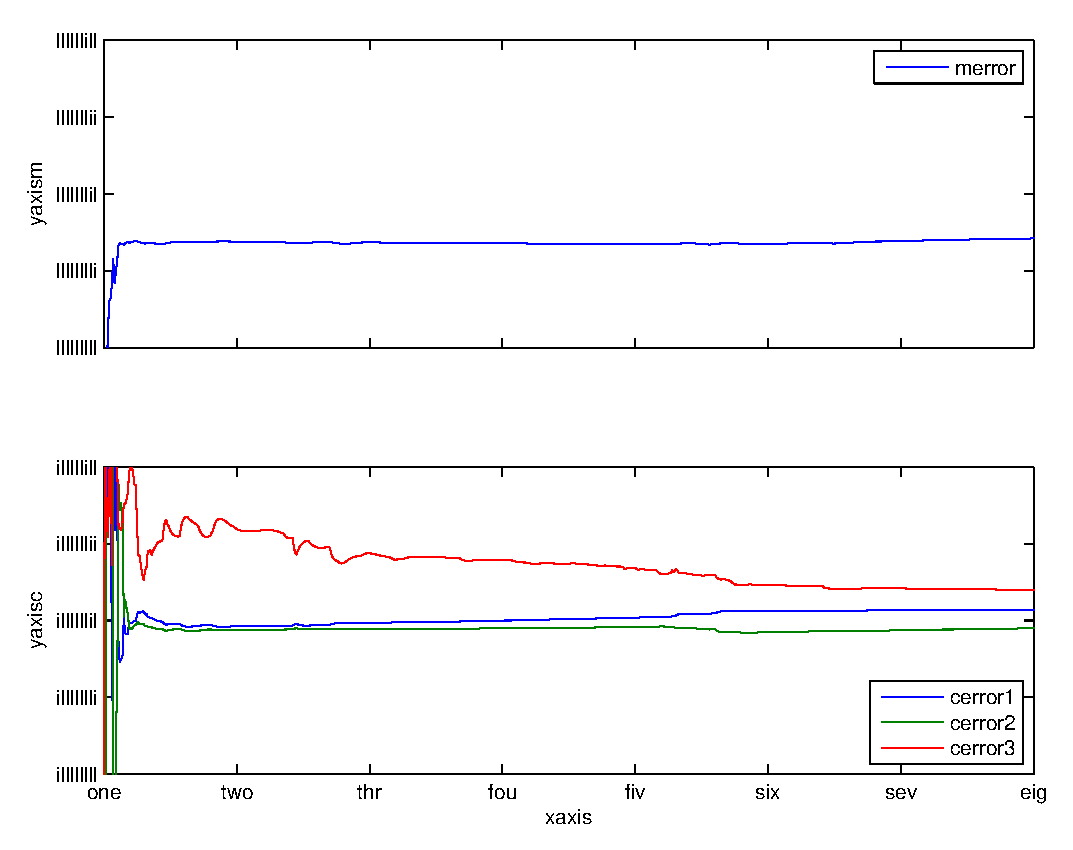
\includegraphics[width=0.6\textwidth]{fig/one_grasping_point_fast_mass_and_cog.eps}
		\end{figure}
		\vspace{0.2cm}
		Error of center of gravity $\vec{c} \left[\mathrm{m}\right]$
	\end{center}
\end{frame}

\begin{frame}
	%Benedikt
	\frametitle{Estimation Results}
	\begin{center}
		\begin{figure}
			\psfrag{xaxis}[tr][br]{$t\left[\mathrm{s}\right]$}
			\psfrag{yaxis}[bc][tr]{}
			\psfrag{one}[c][Bc]{$0$}
			\psfrag{two}[c][Bc]{$1$}
			\psfrag{thr}[c][Bc]{$2$}
			\psfrag{fou}[c][Bc]{$3$}
			\psfrag{fiv}[c][Bc]{$4$}
			\psfrag{six}[c][Bc]{$5$}
			\psfrag{sev}[c][Bc]{$6$}
			\psfrag{eig}[c][Bc]{$7$}
			\psfrag{lllllllll}[Br][Bl]{$-0.02\  $}
			\psfrag{lllllllli}[Br][Bl]{$-0.01\ $}
			\psfrag{lllllllil}[Br][Bl]{$0\  $}
			\psfrag{lllllllii}[Br][Bl]{$0.01\  $}
			\psfrag{llllllill}[Br][Bl]{$0.02\  $}
			\psfrag{Ixxerror}[][]{\tiny $I_{xx}$}
			\psfrag{Iyyerror}[][]{\tiny $I_{yy}$}
			\psfrag{Izzerror}[][]{\tiny $I_{zz}$}
			\psfrag{Ixyerror}[][]{\tiny $I_{xy}$}
			\psfrag{Ixzerror}[][]{\tiny $I_{xz}$}
			\psfrag{Iyzerror}[][]{\tiny $I_{yz}$}
			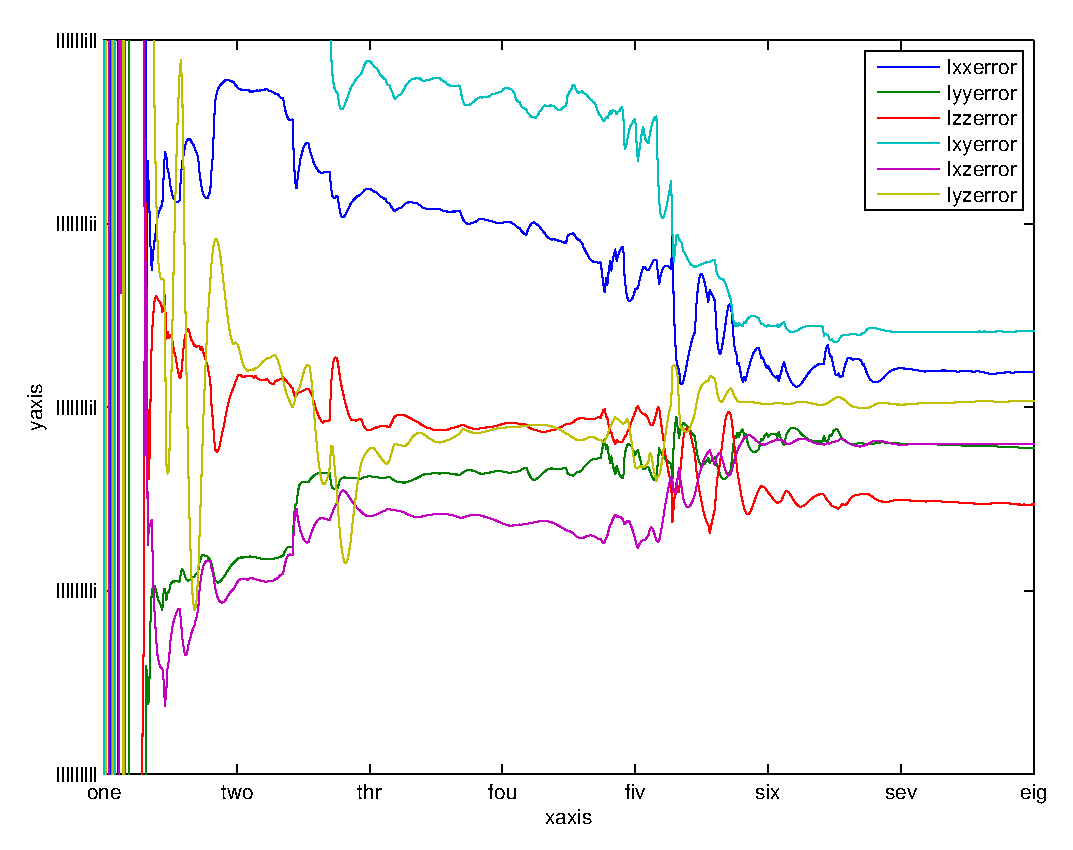
\includegraphics[width=0.6\textwidth]{fig/one_grasping_point_fast_inertias.eps}
		\end{figure}
		\vspace{0.4cm}
		Error of inertias $I \left[\mathrm{kg} \cdot \mathrm{m}^2\right]$
	\end{center}
\end{frame}

\section{Outlook}
\begin{frame}
	%Benedikt
	\frametitle{Remaining Issues}
	\begin{itemize}
		\setlength{\itemsep}{10pt}
		\item Check if input values for the estimator are correct
		\item Find a good excitation pattern
		\item Incorporate human into the identification
	\end{itemize}
\end{frame}
\begin{frame}
	%Benedikt
	\frametitle{Time Schedule}
	\begin{tikzpicture}[node distance=0.2cm]
		\node[shape=circle,fill=green] (A) at (0, 0) {};
		\node[right=of A.east,anchor=west] {Get familiar with the topic and the hardware};
		\node[anchor=west] (DateA) at (0.2, -0.4) {19.11.2014};
		\draw[green,thick] (DateA) -- (A);
		\node[shape=circle,fill=tum_blue] (B) at (0, -1) {};
		\node[right=of B.east,anchor=west] {Implement load identification with one grasping point};
		\node[anchor=west] (DateB) at (0.2, -1.4) {5.12.2014};
		\draw[tum_blue,thick] (DateB) -- (B);
		\node[shape=circle,fill=tum_blue] (C) at (0, -2) {};
		\node[right=of C.east,anchor=west] {Implement load identification with more than one grasping point};
		\node[anchor=west] (DateC) at (0.2, -2.4) {19.12.2014};
		\draw[tum_blue,thick] (DateC) -- (C);
		\node[shape=circle,fill=tum_blue] (D) at (0, -3) {};
		\node[right=of D.east,anchor=west] {Trigger additional excitation by the human through the wrist band};
		\node[anchor=west] (DateD) at (0.2, -3.4) {16.01.2015};
		\draw[tum_blue,thick] (DateD) -- (D);
		\path[top color=green, bottom color=tum_blue, shading path={draw=transparent!0, very thick}] (A.south) -- (B.north);
		\draw[tum_blue,very thick] (B.south) -- (C.north);
		\draw[tum_blue,very thick] (C.south) -- (D.north);
	\end{tikzpicture}
\end{frame}

\appendix
\begin{frame}
	\frametitle{References}
	\printbibliography
\end{frame}

\end{document}
